
\begin{frame}
  \frametitle{In close collaboration with ... }

 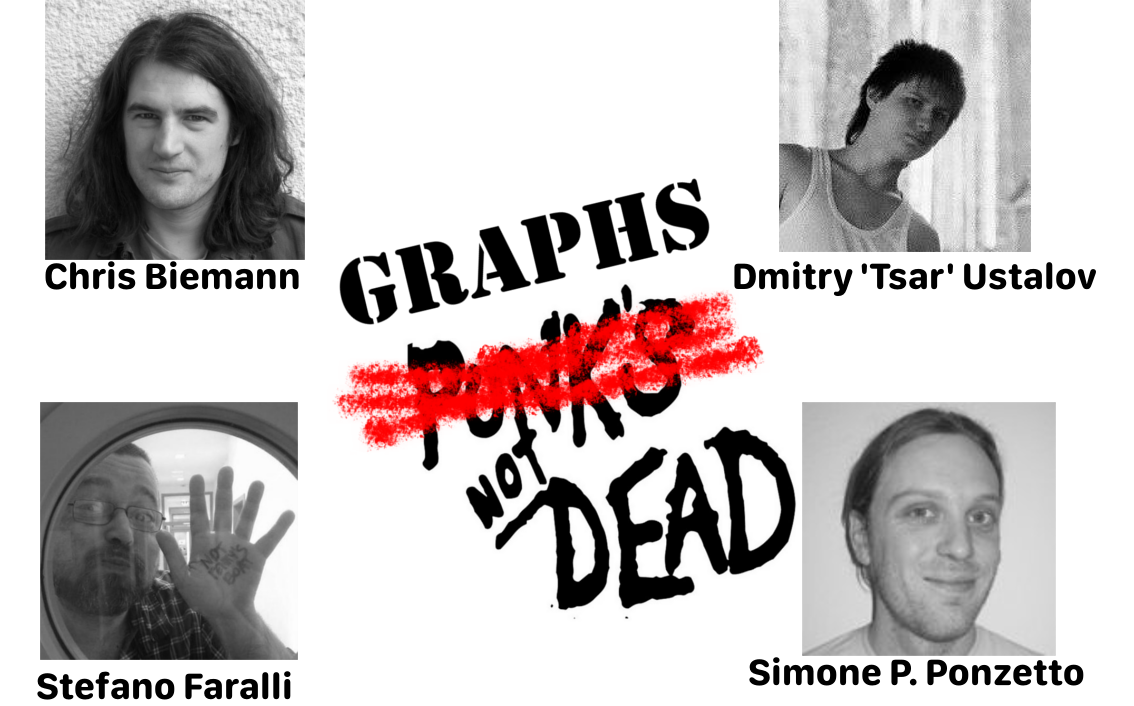
\includegraphics[width=.95\textwidth]{figures/collaborators}	
\end{frame}



\begin{frame}
  \frametitle{In collaboration with ... }
  { \large \bf
  \begin{itemize}
  	\item Andrei Kutuzov
  	\item Eugen Ruppert
  	\item Fide Marten
  	\item Nikolay Arefyev
  	\item Steffen Remus
  	\item Martin Riedl
  	\item Hubert Naets
   	\item Maria Pelevina
	\item Anastasiya Lopukhina
	\item Konstantin Lopukhin
  
  \end{itemize}	
  }
\end{frame}


\section{Overview}

\begin{frame}
  \frametitle{Overview}

  \begin{itemize}
		\item \alert{\textbf{Inducing word sense representations}}:
		\begin{itemize}
		\item \textbf{word sense embeddings via retrofitting} \cite{pelevina-EtAl:2016:RepL4NLP,remus:2018};
		\item \textbf{inducing synsets}~\cite{ustalov-panchenko-biemann:2017:Long,ustalov2017fighting,madoc43362}
		\item \textbf{inducing semantic classes} \cite{panchenko:2018:SemanticClasses} 
				
		\end{itemize}

	
	\pause 
	\vspace{1em}
	\item \alert{\textbf{Making induced senses interpretable}} \cite{panchenko-EtAl:2017:EMNLP2017Demos,panchenko-EtAl:2017:EACLlong}
	
	\pause
	\vspace{1em}
	\item \alert{\textbf{Linking induced word senses to lexical resources}}~\cite{panchenko2016best,faralli2016linked,panchenko-EtAl:2017:SENSE2017,biemann2018framework}	
			
\end{itemize}
	
\end{frame}


\begin{frame}
  \frametitle{Overview}

  \begin{itemize}
  
  			\item \alert{\textbf{A shared task on word sense induction}} \cite{panchenko2018russe,arefyev2018russe}	
  		
  		\pause 	
  		\vspace{10pt}
  
		\item \alert{\textbf{Inducing semantic frames}} \cite{ustalov2018unsupervised} 
		\begin{itemize}
			\item Inducing \textbf{FrameNet}-like structures;
			\item ...using \textbf{multi-way clustering}.
		\end{itemize}
		
		\pause 
		\vspace{10pt} 
		
		\item \alert{\textbf{Learning graph/network embeddings}} [ongoing joint work with Andrei Kutuzov]
		\begin{itemize}
		\item How to \textbf{represent induced networks/graphs}?
		\item ... so that they can be used in \textbf{deep learning architectures}.
		\item ...\textbf{effectively} and \textbf{efficiently}.
		\end{itemize}
		
		 
				
	
			
\end{itemize}
	
\end{frame}



